%==============================================================================
% Chapitre 65 - Synthèse des munitions de chasse
%==============================================================================

\section{Introduction}

Les chapitres précédents ont présenté les principaux composants et
caractéristiques des munitions de chasse.

Cette synthèse permet de rassembler les notions essentielles avant
d'aborder les phénomènes balistiques qui se produisent lors du tir.

\begin{aretenir}

Une cartouche de chasse constitue un système complet dont tous les éléments
interagissent.

\end{aretenir}

\section{Les composants principaux}

Une cartouche de chasse comprend généralement :

\begin{itemize}
    \item une amorce ;
    \item une charge de poudre ;
    \item une bourre ;
    \item une charge de projectiles ;
    \item une douille ;
    \item un sertissage.
\end{itemize}

Chaque composant possède une fonction spécifique.

\begin{figure}[htbp]
\centering

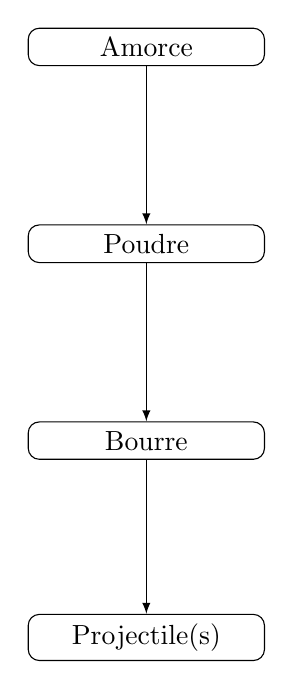
\begin{tikzpicture}[
every node/.style={
draw,
rounded corners,
align=center,
minimum width=3cm
}
]

\node (A) at (0,0)
{Amorce};

\node (P) at (0,-2.5)
{Poudre};

\node (B) at (0,-5)
{Bourre};

\node (Pr) at (0,-7.5)
{Projectile(s)};

\draw[-latex] (A) -- (P);
\draw[-latex] (P) -- (B);
\draw[-latex] (B) -- (Pr);

\end{tikzpicture}

\caption{Chaîne fonctionnelle simplifiée d'une cartouche de chasse.}
\label{fig:chaine_cartouche}

\end{figure}

\section{Les différents types de projectiles}

Les projectiles étudiés peuvent être regroupés en trois grandes familles :

\begin{itemize}
    \item la grenaille ;
    \item les chevrotines ;
    \item les balles.
\end{itemize}

Chaque famille répond à des besoins différents.

\begin{figure}[htbp]
\centering

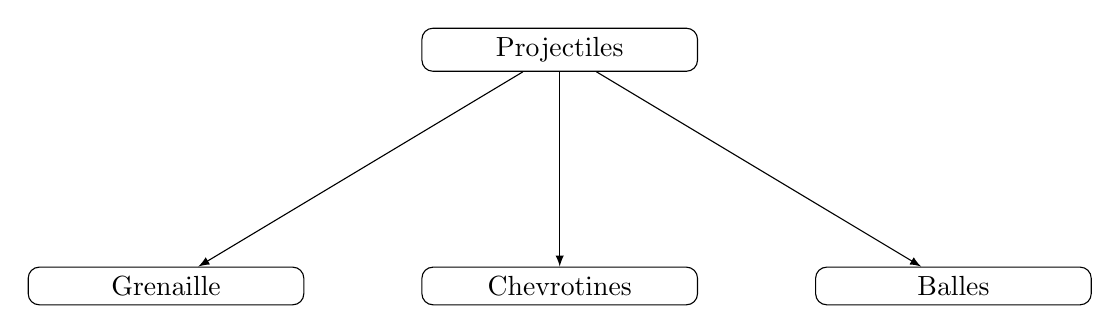
\begin{tikzpicture}[
every node/.style={
draw,
rounded corners,
align=center,
minimum width=3.5cm
}
]

\node (P) at (0,0)
{Projectiles};

\node (G) at (-5,-3)
{Grenaille};

\node (C) at (0,-3)
{Chevrotines};

\node (B) at (5,-3)
{Balles};

\draw[-latex] (P) -- (G);
\draw[-latex] (P) -- (C);
\draw[-latex] (P) -- (B);

\end{tikzpicture}

\caption{Principales familles de projectiles étudiées dans cette partie.}
\label{fig:famille_projectiles}

\end{figure}

\section{Influence de la taille des projectiles}

Le diamètre des projectiles influence directement :

\begin{itemize}
    \item leur masse ;
    \item leur énergie ;
    \item leur portée utile ;
    \item leur comportement terminal.
\end{itemize}

\section{Le rôle de la bourre}

La bourre assure plusieurs fonctions simultanément :

\begin{itemize}
    \item transmission de la poussée ;
    \item étanchéité ;
    \item protection des projectiles ;
    \item influence sur la gerbe.
\end{itemize}

\section{Le rôle du choke}

Le choke agit principalement sur la dispersion de la charge.

Son effet dépend également des munitions utilisées.

\section{La gerbe}

La qualité d'une cartouche à grenaille ne dépend pas uniquement du nombre de
projectiles.

La répartition des impacts constitue également un paramètre fondamental.

\section{Les calibres}

Les calibres de chasse utilisent une convention historique particulière.

Leur désignation ne correspond pas directement au diamètre du canon.

\section{Les matériaux}

Le matériau influence :

\begin{itemize}
    \item la masse ;
    \item la densité ;
    \item le comportement en vol ;
    \item les performances terminales.
\end{itemize}

\section{L'importance des essais}

Les performances réelles dépendent de nombreux paramètres.

Les essais pratiques restent indispensables pour évaluer correctement une
combinaison arme-munition.

\section{Une approche systémique}

Aucun composant ne peut être étudié isolément.

Le comportement observé résulte de l'interaction entre :

\begin{itemize}
    \item l'arme ;
    \item la munition ;
    \item les conditions de tir ;
    \item la cible.
\end{itemize}

\begin{figure}[htbp]
\centering


\begin{tikzpicture}[
every node/.style={
draw,
rounded corners,
align=center,
minimum width=3cm
}
]

\node (Arme) at (0,0)
{Arme};

\node (Mun) at (5,0)
{Munition};

\node (Tir) at (10,0)
{Tir};

\node (Cible) at (15,0)
{Cible};

\draw[-latex] (Arme) -- (Mun);
\draw[-latex] (Mun) -- (Tir);
\draw[-latex] (Tir) -- (Cible);

\end{tikzpicture}

\caption{Le résultat observé dépend de l'ensemble du système de tir.}
\label{fig:systeme_tir}

\end{figure}

\section{Préparer l'étude de la balistique}

Jusqu'à présent, les différents composants ont été étudiés séparément.

La prochaine partie examinera ce qui se produit lorsqu'un coup est tiré.

Les phénomènes étudiés deviendront alors dynamiques.

\section{Du composant au phénomène}

L'amorce, la poudre et le projectile ont été décrits individuellement.

Il reste désormais à comprendre comment ils interagissent pendant quelques
millisecondes pour produire le départ du coup.

\begin{figure}[htbp]
\centering

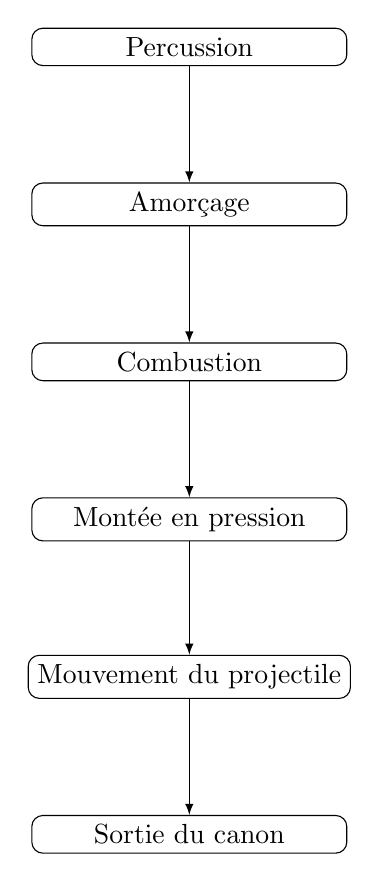
\begin{tikzpicture}[
every node/.style={
draw,
rounded corners,
align=center,
minimum width=4cm
}
]

\node (1) at (0,0)
{Percussion};

\node (2) at (0,-2)
{Amorçage};

\node (3) at (0,-4)
{Combustion};

\node (4) at (0,-6)
{Montée en pression};

\node (5) at (0,-8)
{Mouvement du projectile};

\node (6) at (0,-10)
{Sortie du canon};

\draw[-latex] (1) -- (2);
\draw[-latex] (2) -- (3);
\draw[-latex] (3) -- (4);
\draw[-latex] (4) -- (5);
\draw[-latex] (5) -- (6);

\end{tikzpicture}

\caption{Principales étapes étudiées en balistique intérieure.}
\label{fig:chronologie_depart_coup}

\end{figure}

\section{Transition vers la balistique intérieure}

La balistique intérieure étudie les phénomènes se produisant entre la
percussion de l'amorce et la sortie du projectile de la bouche du canon.

Elle constitue le premier domaine de la balistique dynamique.

\begin{figure}[htbp]
\centering

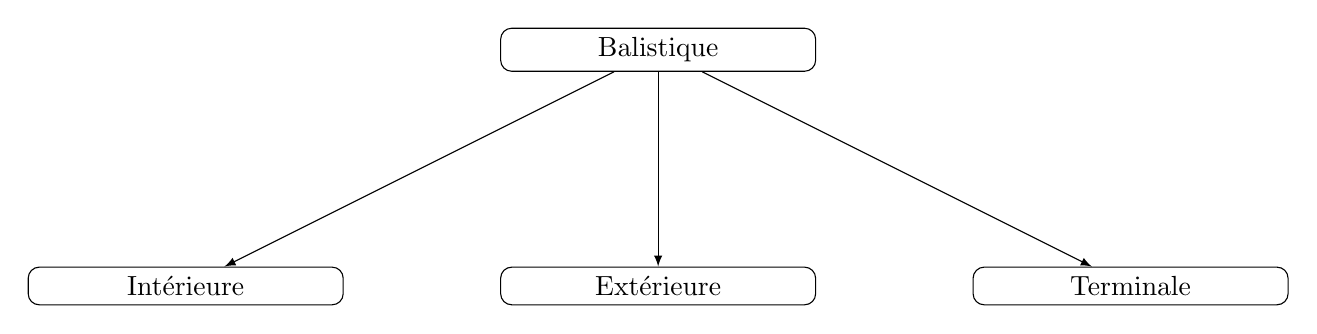
\begin{tikzpicture}[
every node/.style={
draw,
rounded corners,
align=center,
minimum width=4cm
}
]

\node (B) at (0,0)
{Balistique};

\node (I) at (-6,-3)
{Intérieure};

\node (E) at (0,-3)
{Extérieure};

\node (T) at (6,-3)
{Terminale};

\draw[-latex] (B) -- (I);
\draw[-latex] (B) -- (E);
\draw[-latex] (B) -- (T);

\end{tikzpicture}

\caption{Les trois grands domaines de la balistique.}
\label{fig:domaines_balistique}

\end{figure}


\section{À retenir}

\begin{aretenir}

\begin{itemize}
    \item Une munition est un système composé de plusieurs éléments.
    \item Les performances résultent de l'interaction de ces éléments.
    \item La bourre et le choke influencent fortement les gerbes.
    \item Les matériaux et les projectiles modifient le comportement global.
    \item La balistique intérieure étudie ce qui se produit au moment du tir.
\end{itemize}

\end{aretenir}

\begin{figure}[htbp]
\centering

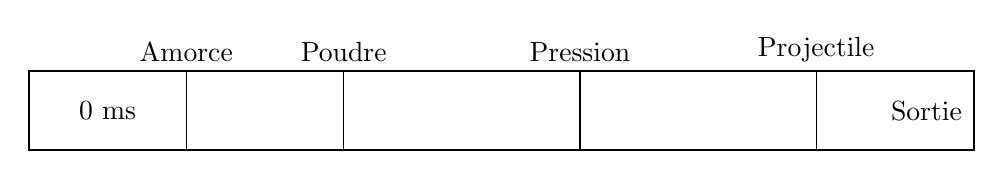
\begin{tikzpicture}[>=latex]

\draw[thick] (0,0) rectangle (12,1);

\node at (1,0.5) {0 ms};

\draw (2,0) -- (2,1);
\node[above] at (2,1) {Amorce};

\draw (4,0) -- (4,1);
\node[above] at (4,1) {Poudre};

\draw (7,0) -- (7,1);
\node[above] at (7,1) {Pression};

\draw (10,0) -- (10,1);
\node[above] at (10,1) {Projectile};

\node at (11.4,0.5)
{Sortie};

\end{tikzpicture}

\caption{Les phénomènes étudiés en balistique intérieure se déroulent sur quelques millisecondes seulement.}
\label{fig:quelques_millisecondes}

\end{figure}
